% ============================================================
\chapter{Variables, Types et Op\'erations de Base}
\label{ch:variables}
% ============================================================

\section{Les variables : des bo\^ites avec des \'etiquettes}

\begin{intuition}
Une \textbf{variable}\index{variable} est comme une bo\^ite \'etiquet\'ee dans laquelle on range une valeur. L'\'etiquette (le nom) permet de retrouver le contenu \`a tout moment.
\end{intuition}

\begin{center}
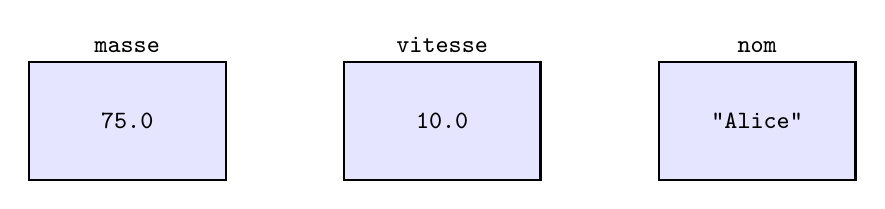
\begin{tikzpicture}
  \foreach \name/\val/\x in {masse/75.0/0, vitesse/10.0/4, nom/{"Alice"}/8} {
    \draw[thick, fill=blue!10] (\x,0) rectangle (\x+2.5,1.5);
    \node[font=\small\ttfamily] at (\x+1.25,0.75) {\val};
    \node[font=\small\ttfamily, above] at (\x+1.25,1.5) {\name};
  }
\end{tikzpicture}
\end{center}

\begin{codeblock}[title=\textbf{Python --- Cr\'eer des variables}]
\begin{minted}{python}
# Créer des variables
masse = 75.0         # nombre décimal (float)
age = 20             # nombre entier (int)
nom = "Alice"        # chaîne de caractères (str)
est_etudiant = True  # booléen (bool)

print(f"Nom : {nom}, Âge : {age}")
print(f"Masse : {masse} kg")
print(f"Étudiant : {est_etudiant}")
\end{minted}
\end{codeblock}

\begin{codeoutput}
\begin{verbatim}
Nom : Alice, Âge : 20
Masse : 75.0 kg
Étudiant : True
\end{verbatim}
\end{codeoutput}

\begin{attention}
En Python, on ne <<~d\'eclare~>> pas le type d'une variable. Python le d\'eduit automatiquement. C'est le \textbf{typage dynamique}\index{typage dynamique}.
\end{attention}

\section{Les types de donn\'ees}

\begin{definition}[Types fondamentaux]\index{types}
Python poss\`ede quatre types fondamentaux :
\begin{itemize}
\item \py{int} --- entier : \py{42}, \py{-7}, \py{0}
\item \py{float} --- d\'ecimal : \py{3.14}, \py{-0.5}, \py{6.022e23}
\item \py{str} --- cha\^ine : \py{"Bonjour"}, \py{'xyz'}
\item \py{bool} --- bool\'een : \py{True}, \py{False}
\end{itemize}
\end{definition}

\begin{codeblock}[title=\textbf{Python --- V\'erifier le type}]
\begin{minted}{python}
x = 42
y = 3.14
z = "physique"
b = True

print(type(x))   # <class 'int'>
print(type(y))   # <class 'float'>
print(type(z))   # <class 'str'>
print(type(b))   # <class 'bool'>
\end{minted}
\end{codeblock}

\begin{codeoutput}
\begin{verbatim}
<class 'int'>
<class 'float'>
<class 'str'>
<class 'bool'>
\end{verbatim}
\end{codeoutput}

\section{Notation scientifique}

\begin{codeblock}[title=\textbf{Python --- Notation scientifique}]
\begin{minted}{python}
# Constantes physiques en notation scientifique
c = 2.998e8        # vitesse de la lumière (m/s)
h = 6.626e-34      # constante de Planck (J·s)
Na = 6.022e23      # nombre d'Avogadro (mol⁻¹)
G = 6.674e-11      # constante gravitationnelle

print(f"c  = {c}")
print(f"h  = {h}")
print(f"Na = {Na}")
print(f"G  = {G}")
\end{minted}
\end{codeblock}

\begin{codeoutput}
\begin{verbatim}
c  = 299800000.0
h  = 6.626e-34
Na = 6.022e+23
G  = 6.674e-11
\end{verbatim}
\end{codeoutput}

\section{Conversion de types}

\begin{codeblock}[title=\textbf{Python --- Conversions}]
\begin{minted}{python}
# int -> float
x = float(42)
print(x, type(x))        # 42.0 <class 'float'>

# float -> int (tronque !)
y = int(3.99)
print(y, type(y))        # 3 <class 'int'>

# str -> int ou float
temperature = int("25")
pi_approx = float("3.14")
print(temperature, pi_approx)

# Nombre -> str
message = "La réponse est " + str(42)
print(message)
\end{minted}
\end{codeblock}

\begin{codeoutput}
\begin{verbatim}
42.0 <class 'float'>
3 <class 'int'>
25 3.14
La réponse est 42
\end{verbatim}
\end{codeoutput}

\section{Op\'erations sur les cha\^ines}

\begin{codeblock}[title=\textbf{Python --- Cha\^ines de caract\`eres}]
\begin{minted}{python}
prenom = "Marie"
nom = "Curie"

# Concaténation
nom_complet = prenom + " " + nom
print(nom_complet)

# Répétition
print("-" * 30)

# Longueur
print(f"Longueur : {len(nom_complet)}")

# Accès par index (commence à 0 !)
print(f"Première lettre : {nom_complet[0]}")
print(f"Dernière lettre : {nom_complet[-1]}")

# Méthodes utiles
print(nom_complet.upper())
print(nom_complet.lower())
print(nom_complet.replace("Curie", "Skłodowska-Curie"))
\end{minted}
\end{codeblock}

\begin{codeoutput}
\begin{verbatim}
Marie Curie
------------------------------
Longueur : 11
Première lettre : M
Dernière lettre : e
MARIE CURIE
marie curie
Marie Skłodowska-Curie
\end{verbatim}
\end{codeoutput}

\begin{center}
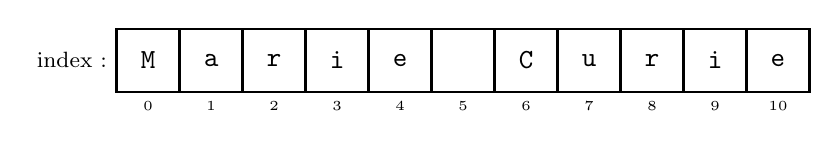
\begin{tikzpicture}
  \foreach \c/\i in {M/0,a/1,r/2,i/3,e/4,{~}/5,C/6,u/7,r/8,i/9,e/10} {
    \draw[thick] (\i*0.8,0) rectangle (\i*0.8+0.8,0.8);
    \node[font=\ttfamily] at (\i*0.8+0.4,0.4) {\c};
    \node[font=\tiny,below] at (\i*0.8+0.4,0) {\i};
  }
  \node[font=\footnotesize,left] at (0,0.4) {index :};
\end{tikzpicture}
\end{center}

\section{Les f-strings (cha\^ines format\'ees)}

\begin{codeblock}[title=\textbf{Python --- f-strings}]
\begin{minted}{python}
element = "Hydrogène"
masse_atomique = 1.008
numero = 1

# f-string : insérer des variables dans du texte
print(f"L'élément {element} (Z={numero}) a une masse de {masse_atomique} u")

# Formatage des nombres
pi = 3.141592653589793
print(f"π = {pi:.2f}")      # 2 décimales
print(f"π = {pi:.6f}")      # 6 décimales
print(f"π = {pi:.2e}")      # notation scientifique

# Alignement
for element, masse in [("H", 1.008), ("C", 12.011), ("O", 15.999)]:
    print(f"{element:<5} {masse:>8.3f} u")
\end{minted}
\end{codeblock}

\begin{codeoutput}
\begin{verbatim}
L'élément Hydrogène (Z=1) a une masse de 1.008 u
π = 3.14
π = 3.141593
π = 3.14e+00
H         1.008 u
C        12.011 u
O        15.999 u
\end{verbatim}
\end{codeoutput}

\section{Op\'erateurs de comparaison et bool\'eens}

\begin{codeblock}[title=\textbf{Python --- Comparaisons}]
\begin{minted}{python}
x = 10
print(x > 5)       # True
print(x == 10)      # True (égalité)
print(x != 7)       # True (différent)
print(x >= 15)      # False

# Opérateurs logiques
a = True
b = False
print(a and b)      # False
print(a or b)       # True
print(not a)        # False
\end{minted}
\end{codeblock}

\begin{codeoutput}
\begin{verbatim}
True
True
True
False
False
True
False
\end{verbatim}
\end{codeoutput}

\begin{formules}[title=\textbf{Op\'erateurs de comparaison}]
\begin{tabular}{lll}
\toprule
\textbf{Op\'erateur} & \textbf{Signification} & \textbf{Exemple} \\
\midrule
\py{==} & \'Egal \`a & \py{5 == 5} $\to$ \py{True} \\
\py{!=} & Diff\'erent de & \py{5 != 3} $\to$ \py{True} \\
\py{<}, \py{>} & Inf\'erieur, sup\'erieur & \py{3 < 5} $\to$ \py{True} \\
\py{<=}, \py{>=} & Inf. ou \'egal, sup. ou \'egal & \py{5 >= 5} $\to$ \py{True} \\
\py{and} & ET logique & \py{True and False} $\to$ \py{False} \\
\py{or} & OU logique & \py{True or False} $\to$ \py{True} \\
\py{not} & NON logique & \py{not True} $\to$ \py{False} \\
\bottomrule
\end{tabular}
\end{formules}

\section{L'entr\'ee utilisateur}

\begin{codeblock}[title=\textbf{Python --- input}]
\begin{minted}{python}
# input() retourne toujours une chaîne !
# nom = input("Votre nom : ")
# age = int(input("Votre âge : "))
# print(f"Bonjour {nom}, vous avez {age} ans.")

# Simulation (pour le cours)
nom = "Alice"
age = 20
print(f"Bonjour {nom}, vous avez {age} ans.")
\end{minted}
\end{codeblock}

\begin{codeoutput}
\begin{verbatim}
Bonjour Alice, vous avez 20 ans.
\end{verbatim}
\end{codeoutput}

\section{Ce qui peut mal tourner}

\begin{errmark}
\begin{codeblock}[title=\textbf{Erreurs fr\'equentes}]
\begin{minted}{python}
# 1. Oublier les guillemets pour les chaînes
# nom = Alice        # NameError: name 'Alice' is not defined
nom = "Alice"        # Correct

# 2. Confondre = (affectation) et == (comparaison)
x = 5                # affecte 5 à x
# x == 5             # compare x à 5, retourne True

# 3. Diviser un entier et attendre un flottant
print(7 / 2)         # 3.5 (en Python 3, ok)
print(7 // 2)        # 3 (division entière !)

# 4. Concaténer un nombre et une chaîne
# print("J'ai " + 20 + " ans")  # TypeError
print("J'ai " + str(20) + " ans")  # OK
print(f"J'ai {20} ans")            # Encore mieux
\end{minted}
\end{codeblock}
\end{errmark}

\section{Mini-projet : Fiche d'identit\'e d'un atome}

\begin{projet}
Cr\'eez un programme qui affiche la fiche d'identit\'e d'un atome.

\begin{codeblock}[title=\textbf{Python}]
\begin{minted}{python}
# Fiche d'identité : Carbone
element = "Carbone"
symbole = "C"
numero_atomique = 6
masse_atomique = 12.011  # u
electronegativite = 2.55  # Pauling

print("=" * 35)
print(f"  FICHE D'IDENTITÉ : {element}")
print("=" * 35)
print(f"  Symbole           : {symbole}")
print(f"  Numéro atomique   : {numero_atomique}")
print(f"  Masse atomique    : {masse_atomique} u")
print(f"  Électronégativité : {electronegativite}")
print(f"  Nombre de protons : {numero_atomique}")
print(f"  Nombre d'électrons: {numero_atomique}")
print("=" * 35)
\end{minted}
\end{codeblock}

\begin{codeoutput}
\begin{verbatim}
===================================
  FICHE D'IDENTITÉ : Carbone
===================================
  Symbole           : C
  Numéro atomique   : 6
  Masse atomique    : 12.011 u
  Électronégativité : 2.55
  Nombre de protons : 6
  Nombre d'électrons: 6
===================================
\end{verbatim}
\end{codeoutput}
\end{projet}

\section{Exercices}

\begin{exercice}[$\star$ --- Guid\'e]
Cr\'eez des variables pour stocker la constante de Boltzmann ($k_B = 1.381 \times 10^{-23}$~J/K) et une temp\'erature $T = 300$~K. Calculez l'\'energie thermique $E = k_B T$ et affichez le r\'esultat.
\end{exercice}

\begin{exercice}[$\star$ --- Guid\'e]
Cr\'eez une variable \py{rayon = 6371} (rayon de la Terre en km). Calculez et affichez la circonf\'erence ($C = 2\pi r$) et la surface ($S = 4\pi r^2$) de la Terre.
\end{exercice}

\begin{exercice}[$\star\star$ --- Ind\'ependant]
\'Ecrivez un programme qui demande \`a l'utilisateur une distance en kilom\`etres et la convertit en miles (1~km $= 0.621$~miles), en m\`etres et en centim\`etres.
\end{exercice}

\begin{exercice}[$\star\star$ --- Ind\'ependant]
Cr\'eez un programme qui calcule l'IMC (Indice de Masse Corporelle) : $\text{IMC} = \frac{\text{masse (kg)}}{\text{taille (m)}^2}$. Affichez le r\'esultat avec 1 d\'ecimale.
\end{exercice}

\begin{exercice}[$\star\star\star$ --- D\'efi scientifique]
La formule de l'\'energie d'un photon est $E = hf = hc/\lambda$. Calculez l'\'energie d'un photon de lumi\`ere rouge ($\lambda = 700$~nm) et de lumi\`ere bleue ($\lambda = 450$~nm). Exprimez les r\'esultats en joules et en \'electron-volts ($1$~eV $= 1.602 \times 10^{-19}$~J).
\end{exercice}

\begin{formules}[title=\textbf{R\'esum\'e du chapitre}]
\begin{itemize}
\item Une variable stocke une valeur : \py{x = 42}.
\item Types : \py{int}, \py{float}, \py{str}, \py{bool}.
\item \py{type(x)} donne le type, \py{int()}/\py{float()}/\py{str()} convertissent.
\item Notation scientifique : \py{6.022e23} = $6.022 \times 10^{23}$.
\item f-strings : \py{f"pi = \{pi:.2f\}"} pour le formatage.
\item Op\'erateurs de comparaison : \py{==}, \py{!=}, \py{<}, \py{>}, \py{and}, \py{or}.
\end{itemize}
\end{formules}
